\documentclass[../main.tex]{subfiles}

\begin{document}
Neuronale Netze werden, wie auch in dieser Arbeit, häufig zur Bild- und Mustererkennung genutzt. Dabei steht dem Netzwerk eine zweidimensionale Matrix von Pixelinformation in Form von Farb- oder Graustufeninformationen als Eingabe zur Verfügung. Aus dieser Eingabe soll nun eine Ausgabe in Form einer Klassifizierung bestimmt werden.  Eine solche Zuordnung kann mit den bereits beschriebenen klassischen Neuronalen Netzen erfolgen. Der Nachteil dieser Methode ist, dass diese Art von Neuronennetzen die innere Struktur der Bilder nicht berücksichtigen können. Beispielsweise stellt eine Verschiebung des Musters innerhalb des Eingangsbildes für solche Netze ein Problem bei der Erkennung dar. Auch eine Verkleinerung oder Vergrößerung führt zu Problemen. Solche Effekte müssen zur zuverlässigen Erkennung bereits in den Trainingsdaten berücksichtigt werden. Dies führt unweigerlich zu größeren Datensätzen, die für das Training eines zuverlässigen Netzes benötigt werden. Dies könnte durch Einbeziehung der inneren Struktur des Bildes verhindert werden. Dazu stellten Yann LeCun, Léon Bottou, Yoshua Bengio und Patrick Haffner in ihrerm Paper \emph{Gradient-based learning applied to document recognition} von 1998 sogenannte \emph{Convolutional Neural Networks} vor. \par Die dort vorgestellte Netzstruktur erlaubt die Erkennung von Strukturen unabhängig von ihrer Position im Ausgangsbild. Im folgenden Abschnitt soll das grundlegende Prinzip von Convolutional Neural Networks (CNN) vorgestellt und erläutert werden.
\section{Faltungsoperation}
Convolutional Neural Networks beruhen auf der mathematischen Faltungsoperation (Convolution). Auf abstrakter Ebene wird des zweidimensionale Eingangsbild $X(i,j)$ mit einem zweidimensionalen gewichteten Fenster $W(k,l)$ gefaltet. 
\begin{align}
	Y(i,j) = \sum\limits_{p=0}^{n}\sum\limits_{q=0}^{n} X(i-p+a,j-q+a)W(p,q) \label{eq:faltung_math}
\end{align}
Gleichung \ref{eq:faltung_math} zeigt die diskrete Faltung für den genannten Fall. Dabei bezeichnet $n$ die Zeilen- bzw. Spaltenzahl der quadratischen Matrix $W$ und $a$ einen von $n$ abhängigen Parameter, der das Fenster korrekt positioniert. Bildlich gesprochen wird hier ein gewichtetes Fenster sowohl in horizontaler als auch in vertikaler Richtung über das Ausgangsbild bewegt. An jeder Position werden die jeweiligen Werte des Ausgangsbildes mit den gewichten der Fenstermatrix multipliziert und zu einem Wert addiert. Dieser Wert fließt in Convolutional Neural Networks in ein Neuron der nächsten Netzwerkschicht.\par
\begin{figure}[!htbp]
	\centering
	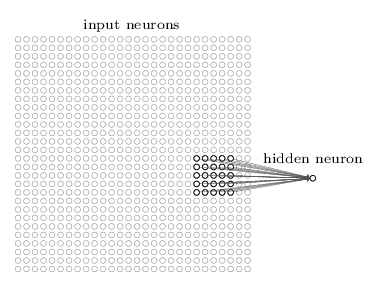
\includegraphics[width=0.8\linewidth]{../images/Riedle/Convolution_1}
	\caption{Berechnung eines Neurons aus einem Faltungskern (vgl. \cite{NNADL_PIC_CONV_1})} \label{fig:conv_1}
\end{figure} 
In Abbildung \ref{fig:conv_1} ist der Vorgang für den Faltungskern an einer Position dargestellt. Dabei werden Neuronen aus dem Eingangsbild über den Faltungskern mit den entsprechenden Gewichten auf ein Hidden Neuron abgebildet. \par 
\begin{figure}[!htbp]
	\centering
	\begin{subfigure}{0.5\textwidth}
		\centering
		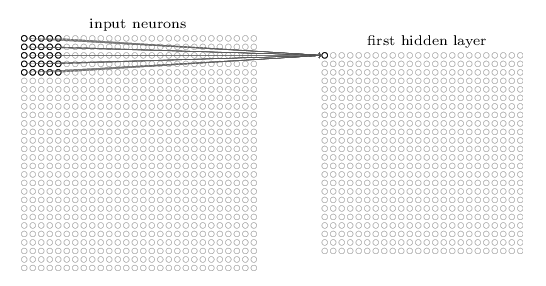
\includegraphics[width=0.8\linewidth]{../images/Riedle/Convolution_2_1}
	\end{subfigure}%
	\begin{subfigure}{0.5\textwidth}
		\centering
		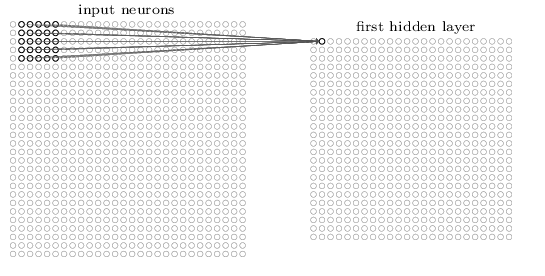
\includegraphics[width=0.8\linewidth]{../images/Riedle/Convolution_2_2}
	\end{subfigure}
	\caption{Faltungsoperation für zwei Ausgangsneuronen (vgl. \cite{NNADL_PIC_CONV_2})} \label{fig:conv_2}
\end{figure}
Führt man nun die Faltung weiter, erhält man als Ergebnis erneut ein zweidimensionales Ausgangsbild mit geringerer Seitenlänge. Abbildung \ref{fig:conv_2} zeigt diesen Schritt. Für ein $28\times28$-Eingangsbild und einen $5\times5$-Faltungskern erhält man bei einer Schrittweite von $1$ beispielsweise ein $24\times24$-Ausgangsbild. \par 
Bei dieser Faltungsoperation werden logischerweise für jedes Neuron die gleichen Gewichte verwendet. Im Fall des hier gezeigten Neuronalen Netzwerkes teilen sich die Ausgangsneuronen dieser Operation auch die Biases. Mit der Aktivierungsfunktion $\sigma$ bestimmt sich der Output eines Neurons damit nach Gleichung \ref{eq:conv_activation}.
\begin{align}\label{eq:con_activation}
	output = \sigma(b+ \sum\limits_l\sum\limits_m w_{l,m}a_{j+l,k+m})
\end{align} \par
Mit einem Satz geteilter Gewichte und Biases ist das Netz nun in der Lage, ein Strukturelement an beliebigen Positionen im Bild zu erkennen. Um es dem Netz nun zu gestatten, mehrere verschiedene Strukturen zu erkennen, vervielfacht man diesen Vorgang mit je eigenen Gewichten und Biases. Es entstehen sogenannte Featuremaps.
\begin{figure}[!htbp]
	\centering
	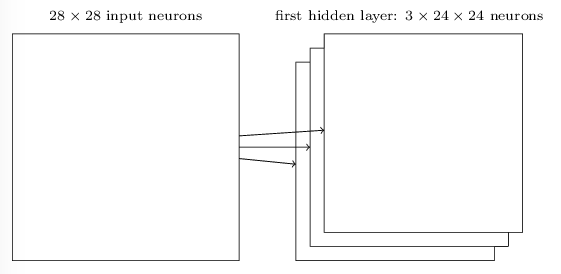
\includegraphics[width=0.8\linewidth]{../images/Riedle/Convolution_Features}
	\caption{Darstellung verschiedener Featuremaps (vgl. \cite{NNADL_PIC_CONV_FEATURES})} \label{fig:conv_features}
\end{figure}
Dieser Vorgang ist in Abbildung \ref{fig:conv_features} dargestellt. Das Netzwerk ist somit in der Lage verschiedene Strukturelemente an beliebigen Positionen zu erkennen. Erweitert man das Netz um weitere Schichten, kann es mit entsprechendem Training auch lernen, welche Kombinationen dieser Elemente zu einem Mustertyp gehören.\par Damit erweitert sich der eingangs genannte Vorteil von CNNs. Nicht nur die Verschiebung ganzer Muster innerhalb eines Bildes kann erkannt werden, sondern auch wiederkehrende Strukturelemente können für die Erkennung anderer Muster durch entsprechende Kombination in weiteren Schichten genutzt werden.
\section{Pooling}
Die Erzeugung von vielen Featuremaps aus einer einzelnen Eingabe gehört zu den grundlegenden Eigenschaften der im vorherigen Abschnitt beschriebenen Faltungsoperation. Dies führt allerdings zu einer erheblichen Vergrößerung der Datenmenge, die von nachfolgenden Layern bearbeitet werden muss. Um das Ausmaß dieser Vergrößerung einschätzen zu können, wird an dieser Stelle die Größe des Outputs einer Faltung in Abhängigkeit von der Eingabegröße und weiterer Eigenschaften der Faltungsschicht untersucht. 
In den nachfolgenden Gleichungen steht \(S\) für die Größe einer einzelnen Ein- bzw. Ausgabe. Die Variablen \(x\), \(y\) und \(f\) stehen für die Dimensionen der Ein- bzw. Ausgabe. Die Größe des Filterkernels ist durch \(F_x\) und \(F_y\) bestimmt, für die Schrittweite wird der Wert \(1\) angenommen. 
\begin{equation}
\begin{split}
S_{in} &= x_{in} y_{in} f_{in}\\
S_{out} &= x_{out} y_{out} f_{out}\\
x_{out} &= x_{in} - F_x + 1\\
y_{out} &= y_{in} - F_y + 1
\end{split}
\end{equation}
Unter der Bedingung, dass \(x_{in} >> F_x\) und \(y_{in} >> F_y\) ergibt sich die Näherung \(\frac{S_{out}}{S_{in}} = \frac{f_{out}}{f_{in}}\). Die Anzahl der Neuronen einer Faltungsschicht gegenüber der des vorherigen Layers steigt bei der Faltungsoperation demzufolge annähernd proportional zur Anzahl der Featuremaps. 
Mit der Datenmenge im Ausgang der Faltungsschicht steigt auch die Zahl der Aktivierungen, die in den nachfolgenden Schichten bearbeitet werden müssen. Dies stellt einen beträchtlichen Mehraufwand dar und kann zu einer signifikanten Steigerung der Rechenzeit und des Speicherbedarfs führen. Um diesen Mehraufwand zu reduzieren, sind die Faltungsschichten in den meisten Implementierungen von CNNs von sogenannten Pooling-Schichten gefolgt. Beim Pooling wird jede Featuremap in rechteckige Abschnitte unterteilt, die dann jeweils auf einen neuen Aktivierungswert abgebildet werden. Für diese Abbildung gibt es mehrere Methoden, einige davon werden im folgenden Abschnitt näher erläutert. 
\subsection{Average Pooling}
Beim Average Pooling wird das arithmetische Mittel aller betrachteten Aktivierungen des Eingangs berechnet. Das Ergebnis wird direkt als Ausgang übernommen. Auf die Verwendung einer Aktivierungsfunktion wird verzichtet, da das Ergebnis durch die Verwendung des arithmetischen Mittels sowieso im für die Aktivierungsfunktion des letzten Layers üblichen Zahlenbereich liegt. Demnach gilt für die Vorwärtsberechnung eines Average Pooling Layers: 
\begin{equation} \label{eq:averagepooling}
output_{x, y} = \frac{\sum\limits_{(m, n)\in{M_x}\times{N_y}} input_{m, n}}{|M_x\times{N_y}|}
\end{equation}
Die Mengen \(M_x\) und \(N_y\) beinhalten dabei jeweils die x- und y-Koordinaten der Eingaben aus dem relevanten Bereich. Die Inhalte dieser Mengen hängen von x bzw. y ab, somit lässt sich jeder Position in der Ausgabe ein eigener Eingabebereich zuordnen. 
\subsection{Max Pooling} \label{maxpool_forward}
Beim Max Pooling werden die betrachteten Aktivierungen des Eingangs miteinander verglichen und der größte Wert wird unverändert im Ausgang übernommen. Auch hier wird auf die erneute Anwendung einer Aktivierungsfunktion verzichtet. Formal lässt sich Max Pooling wie folgt beschreiben: 
\begin{equation} \label{eq:maxpooling}
output_{x, y} = max( {input_{m,n} | m \in M_x; n \in N_y})
\end{equation}
Die obige Gleichung wirkt zwar auf menschliche Betrachter einfach, allerdings ist sie maschinell nicht ohne Schwierigkeiten zu lösen. Der Grund dafür ist, dass zur Berechnung der max-Operation Verzweigungen nötig sind. Bei den meisten modernen CPU-Archtikturen werden diese deutlich langsamer ausgeführt als rein sequentielle Operationen. 
\section{Anpassungen der Backpropagation}
Das Verhalten eines Pooling Layers weicht deutlich vom Verhalten anderer Layertypen ab. Diese Abweichung macht es erforderlich, die zur Backpropagation erforderliche Fehlerweitergabe für diesen Layertyp gesondert zu betrachten. Partielle Ableitungen der Kostenfunktion nach den Gewichten sind an dieser Stelle nicht erforderlich, da weder Average Pooling, noch Max Pooling auf Gewichte zurückgreifen. Zwar existieren auch gewichtsbehaftete Poolingverfahren, (vgl. \cite{paperMixedPooling}) allerdings sind diese nicht Gegenstand dieser Arbeit. Für die Backpropagation eines Pooling Layers ist es also nur erforderlich, die partielle Ableitung der Kostenfunktion nach allen Eingaben zu bestimmen. Da sich die hier behandelten Verfahren deutlich voneinander unterscheiden, werden sie im Folgenden getrennt betrachtet. 
\subsection{Average Pooling}
Die Gleichung \ref{eq:pooling_backprop_std} dient als Ausgangspunkt zur Bestimmung der gesuchten partiellen Ableitung. Wie allgemein bei der Backpropagation gilt auch hier: 
\begin{equation} \label{eq:pooling_backprop_std}
\frac{\partial C}{\partial x_i} = \sum\limits_{j} \frac{\partial C}{\partial y_j} \dot \frac{\partial y_j}{\partial x_i}
\end{equation}
Hier bezeichnet \(C\) das Ergebnis der Kostenfunktion, \(y_j\) alle einzelnen Aktivierungen am Ausgang des Pooling Layers und \(x\) eine beliebige Aktivierung am Eingang des Layers. Die Werte \(\frac{\partial C}{\partial y_j}\) sind nach der Backpropagation in der nachfolgenden Schicht bereits bekannt. \(\frac{\partial C}{\partial x_i}\) muss für jede Eingabe bestimmt werden, damit die Backpropagation im vorherigen Layer fortgesetzt werden kann. Die partiellen Ableitungn \(\frac{\partial y_j}{\partial x_i}\) muss dazu noch bestimmt werden. Zur Vereinfachung wird angenommen, dass sich die rechteckigen Poolingbereiche nicht überschneiden. Dies ist bei dem in dieser Arbeit verwendeten Modell der Fall, allerdings ist es nicht allgemein erforderlich. Mit dieser Vereinfachung ergibt sich, dass es zu jedem \(x_i\) nur ein \(y_j\) gibt, das von ebendiesem \(x_i\) abhängt, für das die Ableitung also nicht \(0\) ist. Darüber hinaus lässt sich zu jedem \(x_i\) eindeutig ein \(y_j\) bestimmen, das weiter betrachtet werden muss. Damit reduziert sich die obige Gleichung auf:
\begin{equation} \label{eq:pooling_backprop_simplified}
\frac{\partial C}{\partial x_i} = \frac{\partial C}{\partial y_j} \dot \frac{\partial y_j}{\partial x_i}
\end{equation}
Der Zusammenhang zwischen \(x_i\) und \(y_j\) ergibt sich aus der Gleichung \ref{eq:averagepooling}, wobei \(x_i\) und \(y_j\) nicht den Koordinaten, sondern stattdessen den Aktivierungen \(input_{m, n}\) bzw. \(output_{x, y}\) entsprechen. Durch Einsetzen ergibt sich also: 
\begin{equation}
y_j = \frac{\sum\limits_{k} x_k}{|M\times{N}|}
\end{equation}
Der Betrag des Kreuzprodukts im Nenner entspricht der Anzahl der Aktivierungen des mit \(y_j\) betrachteten Clusters im Eingang. Wird nun die partielle Ableitung \(\frac{\partial y_j}{\partial x_i}\) gebildet, so fallen alle Summanden außer \(x_k mit k=i\) weg. Dieser Summand wird durch den konstanten Betrag der Clustergröße dividiert, somit ergibt sich für die Ableitung
\begin{equation}
\frac{\partial y_j}{\partial x_i} = \frac{1}{|M\times{N}|}
\end{equation}
Durch Einsetzen in Gleichung \ref{eq:pooling_backprop_simplified} ergibt sich damit die finale Gleichung zur Backpropagation beim Average Pooling: 
\begin{equation} \label{eq:pooling_backprop_avg_final}
\frac{\partial C}{\partial x_i} = \frac{\partial C}{\partial y_j} \dot \frac{1}{|M\times{N}|}
\end{equation}
Wird die Eingabe also in gleich große Cluster eingeteilt, so lässt sich der Fehler aller Aktivierungen im Eingang bestimmen, indem der Fehler der zugehörigen Ausgangsaktivierung duch die konstante Clustergröße dividiert wird. 
\subsection{Max Pooling}
Wie zuvor beim Average Pooling gilt auch hier die Gleichung \ref{eq:pooling_backprop_std}. Außerdem wird wieder angenommen, dass sich die Cluster nicht überschneiden, womit auch Gleichung \ref{eq:pooling_backprop_simplified} ohne Änderungen auf Max Pooling übertragen werden kann. Die Ableitung \(\frac{\partial y_j}{\partial x_i}\) muss allerdings neu bestimmt werden, da sich die beiden Verfahren bei der Vorwärtsberechnung unterscheiden. 
Die Vorwärtsberechnung für Max Pooling ist bereits durch Gleichung \ref{eq:maxpooling} formalisiert. Zunächst wird diese Gleichung unter Verwendung der Variablen \(x_i\) und \(y_j\) neu formuliert. Damit ergibt sich: 
\begin{equation}
y_j = max( {x_k | k \in (M_j \times N_j)})
\end{equation}
Der Index k steht in dieser Gleichung für alle möglichen Positionen von Eingaben in dem für die Ausgangsaktivierung \(y_j\) relevanten Cluster. Wie sich erkennen lässt, hat nur der größte betrachtete Eingang einen Einfluss auf das Ergebnis. Dies macht eine Fallunterscheidung bei der Bestimmung der Ableitung \(\frac{\partial y_j}{\partial x_i}\) notwendig: 
\begin{equation}
   \frac{\partial y_j}{\partial x_i} = 
   \begin{cases}
     1 \text{für } x_i = max( {x_k | k \in (M_j \times N_j)}) \\
     0 \text{sonst}
   \end{cases}
\end{equation}
Dies lässt sich in die zuvor bestimmte Gleichung \ref{eq:pooling_backprop_simplified} einsetzen. Dadurch ergibt sich die finale Gleichung zur Backpropagation beim Max Pooling: 
\begin{equation} \label{eq:pooling_backprop_max_final}
   \frac{\partial C}{\partial x_i} = 
   \begin{cases}
     \frac{\partial C}{\partial y_j} \text{für } x_i = max( {x_k | k \in (M_j \times N_j)}) \\
     0 \text{sonst}
   \end{cases}
\end{equation}
Wie zu erkennen ist, wird hier das Ergebnis der Vorwärtsoperation erneut verwendet. Die Position des Maximums kann daher zwischengespeichert werden, um den Aufwand für eine erneute Berechnung einzusparen. 
\section{Vergleich}
Sowohl Average Pooling, als auch Max Pooling erfüllen die Hauptanforderungen an eine Pooling-Schicht, nämlich eine Datenreduktion um einen durch die Clustergröße bestimmbaren Faktor. Unterschiede zwischen den beiden Verfahren zeigen sich in der Effizienz der Berechnung und der Qualität des Ergebnisses. 
\subsection{Effizienz}
Die Gleichung der Max-Pooling-Operation beinhaltet einen Operator zur Bestimmung des Maximums aus einer Eingabemenge. Wie bereits in Abschnitt \ref{maxpool_forward} erwähnt, ist die maschinelle Berechnung dieses Operators sehr ineffizient. Beim Average Pooling sind zwar mehr Rechenoperationen erforderlich, allerdings lassen sich diese mithilfe moderner CPUs und GPUs deutlich schneller berechnen. Dies ist möglich, weil viele Architekturen Möglichkeiten bereitstellen, gleichartige Operationen gleichzeitig mit einer größeren Menge von Operanden durchzuführen. 
Darüber hinaus benötigt ein Max Pooling Layer zusätzlichen Speicher, um die Position des im Forward-Schritt ermittelten Maximums bis zur Backpropagation zwischenzuspeichern. Bei Prozessoren, die einen Cache besitzen, erhöht zusätzlicher Speicherbedarf die Wahrscheinlichkeit, dass im Cache abgelegte Daten überschrieben werden und erneut aus dem langsameren Arbeitsspeicher gelesen werden müssen. 
Zusammenfassend lässt sich daher feststellen, dass die Berechnung von Average Pooling im Gegensatz zu Max Pooling auf den in dieser Arbeit verwendeten Architekturen performanter ausgeführt wird. Wie groß der tatsächliche Unterschied ist, hängt stark von den verwendeten Prozessoren und Implementierungen ab und lässt sich somit nicht allgemein feststellen. 
\subsection{Qualität}
Die Qualität des Ergebnisses einer Pooling-Operation hängt nicht nur von der Art der Operation selbst, sondern auch von der Art und Aufgabe des Modells, sowie den Eingabedaten ab. Tendenziell hat sich für die meisten bekannten Anwendungen im Bereich der Bildklassifizierung herausgestellt, dass Max Pooling bessere Ergebnisse liefert als Average Pooling. 

Grund für diese Tendenz ist, dass sich die Ausgaben der beiden Verfahren bezüglich ihres Kontrastverhaltens unterscheiden. In den meisten Fällen geht dem Pooling Layer ein Convolution Layer voraus. Bei der Faltungsoperation wird nach bestimmten Bildabschnitten gesucht, die durch einen oder mehrere Filterkernel definiert sind. Wenn der gesuchte Bildabschnitt genau unter dem Filterkernel liegt, schlägt die Aktivierung des Perceptrons für diese Position stark aus. Bereits bei geringen Abweichungen passiert dies allerdings nicht mehr. Stattdessen stellt sich an diesen Positionen ein scheinbar zufälliges Rauschen ein. Bei der nachfolgenden Pooling-Operation sollen die starken Ausschläge möglichst erhalten bleiben, weil darin vermutlich die relevantesten Informationen enthalten sind. Beim Average Pooling werden nun die Featuremaps ähnlich wie mit einem Glättungsfilter derart verarbeitet, dass der Kontrast abnimmt. Somit nähern sich die Ausschläge und das Rauschen signifikant an, wodurch das Ergebnis des Poolings für nachfolgende Layer schwerer zu Verarbeiten wird. Beim Max Pooling werden positive Ausschläge unverändert weitergegeben, somit sind sie auch in nachfolgenden Layern deutlich vom Rest der Featuremap zu unterscheiden. 
Aufgrund der bereits in vorhergenhenden Arbeiten festgestellten besseren Qualität der Ergebnisse bei der Klassifizierung von Ziffern aus der MNIST-Datenbank wird in dieser Arbeit Max Pooling verwendet. 
\end{document}